%Architecture
\subsection{Buts principaux}
%~~~~~~~~~~~~~~~~~~~~~~~~~~~~~~~~~~~~~~~~~~~~~~~~~~~~~~~~~~~~
L'architecture hardware du robot a pour objectif d'être modulable. Cette solution a été retenue afin de pouvoir ajouter des fonctionnalités supplémentaires au cours du projet. L'avantage principal est d'avoir la possibilité de se concentrer sur un module à la fois.

\noindent Quatre modules ont été définis pour permettre au robot de réaliser les actions de bases. Chacun, basé sur une carte électronique propre, sera connecté à la carte principale via un bus de communication (I2C, SPI ou UART). Les modules sont les suivants :

\begin{itemize}
	\item Arduino Master : carte principale qui contrôlera l'ensemble du robot. Elle est à la tête de toutes les autres cartes.;
	\item Arduino Motor : module très important qui commandera les moteurs ;
	\item Raspberry Pi : module qui aura  pour but de voir ce qu'il se passe autour du robot afin de définir les objectifs à atteindre.;
	\item Arduino Bras : carte secondaire qui contrôlera la pince du robot.
\end{itemize}

\paragraph{}
Le fait que l'architecture soit modulable permettra également aux futurs utilisateurs de récupérer un ou plusieurs module pour les exploiter dans leur projet.

\noindent On peut voir les liens entre les différents modules sur la figure~\ref{img:hardware}. On y voit également des éléments tels que la batterie, les moteurs, ou encore les différents capteurs présents sur le robot. Il faut cependant bien avoir en tête que ce schéma n'est qu'une version provisoire qui évoluera avec le projet.

\begin{figure}[!ht]
	\centering
	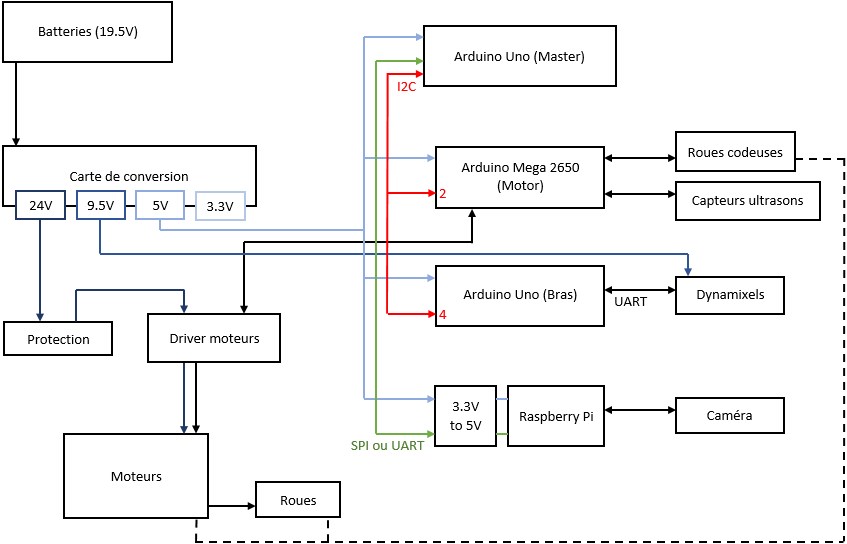
\includegraphics[width=15cm]{hardware.PNG}
	\caption{Schéma bloc hardware}
	\label{img:hardware}
\end{figure}

\subsection{Choix des cartes}
%~~~~~~~~~~~~~~~~~~~~~~~~~~~~~~~~~~~~~~~~~~~~~~~~~~~~~~~~~~~~
Pour notre robot, nous avons ensemble énuméré les avantages et désavantages de chacune des cartes pour nous faciliter la tâche quand nous devrons les utiliser.

\noindent On peut travailler avec une Rasperry Pi, une Arduino ou encore une DE0 nano, mais quelle est la meilleure ? 

\subsubsection{DE0 nano}
%~~~~~~~~~~~~~~~~~~~~~~~~~~~~~~~~~~~~~~~~~~~~~~~~~~~~~~~~~~~~
\noindent Avantages :
\begin{itemize}
	\item Instantanée;
	\item Carte plus performante que les autres (très puissante);
	\item Nombreuses pins à disposition.
\end{itemize}

\noindent Inconvénients :
\begin{itemize}
	\item Difficulté lors de la programmation (VHDL);
	\item Coût important;
	\item Test Bench à faire manuellement;
	\item Limitée par le nombre de sorties;
	\item Temps de compilation plus lent que les autres cartes.
\end{itemize}

\subsubsection{Raspberry Pi}
%~~~~~~~~~~~~~~~~~~~~~~~~~~~~~~~~~~~~~~~~~~~~~~~~~~~~~~~~~~~~
\noindent Avantages :
\begin{itemize}
	\item Utilisation facile, architecture linux;
	\item Utilisation de la caméra aisée;
	\item OpenCV, très bien documenté.
	\item Elle freeze (Testé en laboratoire).
\end{itemize}

\noindent Inconvénients :
\begin{itemize}
	\item Limitation du nombre pins, besoin d'une carte supplémentaire;
	\item Système exploitation, implique que l'on est pas en temps réel; 
	
\end{itemize}

\subsubsection{Arduino}
%~~~~~~~~~~~~~~~~~~~~~~~~~~~~~~~~~~~~~~~~~~~~~~~~~~~~~~~~~~~~
\noindent Avantages :
\begin{itemize}
	\item Consommation faible : 42mA (0,5W) pour 700mA (3,5W) sur Rpi;
	\item Temps réel (ATmega328 8 bits d'Atmel à 16MHz);
	\item Communautaire et très documentée sur internet;
	\item Programmation aisée en C++;
	\item Communication : module pré-existant.
\end{itemize}

\noindent Inconvénients :
\begin{itemize}
\item 32 Ko d'espace mémoire uniquement (Uno);
\item Impossibilité d'intégrer un module caméra avec une Arduino.
\end{itemize}

\subsection{Nomenclature}
%~~~~~~~~~~~~~~~~~~~~~~~~~~~~~~~~~~~~~~~~~~~~~~~~~~~~~~~~~~~~
Cette liste nous permet d'avoir une vue d'ensemble de ce que nous allons utiliser comme matériel. Cependant, elle n'est pas définitive. En effet, elle sera sujette à quelques modifications (ajout et/ou suppression d'éléments) tout au long du projet. 

\noindent Liste : 
\begin{enumerate}
	\item Roues : 
	\begin{itemize}
		\item 2 roues;
		\item 2 roues codeuses;
		\item Buffer 3,3-5V;
		\item Roue libre.
	\end{itemize}

	\item Moteur : 
	\begin{itemize}
		\item 2 moteurs;
		\item 4 engrenages;
		\item 2 courroies;
		\item Drivers.
	\end{itemize}

	\item  Cartes : 
	\begin{itemize}
		\item Raspberry Pi;
		\item 2 Arduino Uno;
		\item DE0 nano;
		\item Arduino Mega 2560;
		\item Carte ECAM RPI (Buffer);
		\item Carte stratégie, initialisation et démarrage avec corde;
		\item Bouton arrêt urgence.
	\end{itemize}

	\item Alimentation : 
	\begin{itemize}
		\item Carte ECAM.
	\end{itemize}

	\item Capteurs : 
	\begin{itemize}
		\item Line tracking;
		\item 2 Gyroscopes accéléromètre;
		\item 5 Capteurs ultrasonique.
	
	\end{itemize}

	\item Châssis : 
	\begin{itemize}
		\item Vis (quincaillerie);
		\item 3 plaques acier;
		\item Tiges;
		\item Courroie-Poulie;
		\item Plexiglas (carrosserie). 
	\end{itemize}

	\item Système levage pince : 
	\begin{itemize}
		\item Pince modèle ECAM ;
		\item Rail ;
		\item 3 Dynamixel;
		\item 2 poulies crantée avec roulement à billes;
		\item Courroie crantée;
		\item 1 plaque en L pour fixer la Dynamixel du la courroie sur structure.
	\end{itemize}
\end{enumerate}